\section{Implementation}

\subsection{Introduction of the systems used}

For the first implementation of basic filtering operations, the evaluation board \textit{Nucleo-H743ZI} of STMicroelectronics
is used. The breakout board \textit{PmodI2S Stereo IN/OUT} is used in order to sample audio data from a 3,5\,mm jack input.

The choice for the \ac{IDE} fell on the
\newline \textit{STM32CubeIDE} as it provides an easy to use installation and
development process.

Digital filters need filter coefficients. For the first approach these
coefficients where computed beforehand and then stored in the memory of the microcontroller. For these computations,
own Python scripts were developed.

In order to design the \ac{PCB}, the \ac{EDA}-software \textit{KiCAD} was used.

\subsection{Implementation of the filters}

As the goal is to develop a variable bandpass filter, not only a set of coefficients for one filter has to be stored,
but many versions of this filter with different mid-frequencies.

As a reference, the frequency response of \textit{Cry-Baby}-Pedal of Prof. Litzenburger has been measured, this is
shown in \autoref{fig:wahwah-filter}.

\begin{figure}[!h]
    \centering
    \begin{subfigure}[c]{0.45\textwidth}
        \centering
        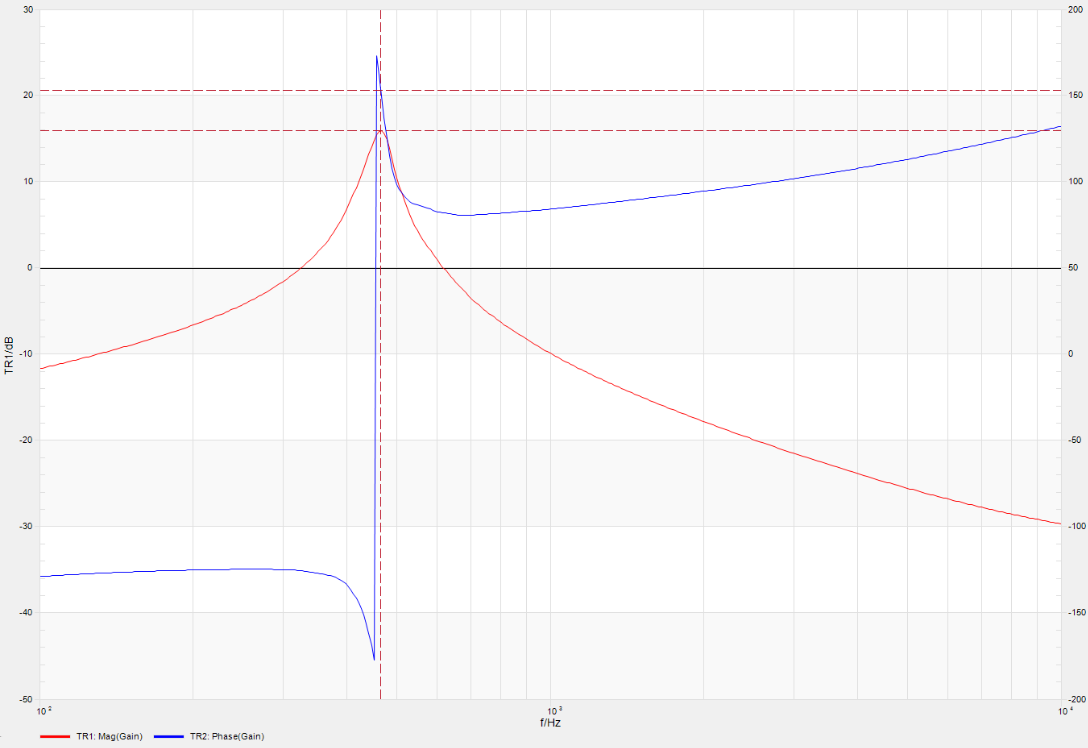
\includegraphics[width=\textwidth]{img/wahwah-1.png}
    \end{subfigure}
    \begin{subfigure}[c]{0.45\textwidth}
        \centering
        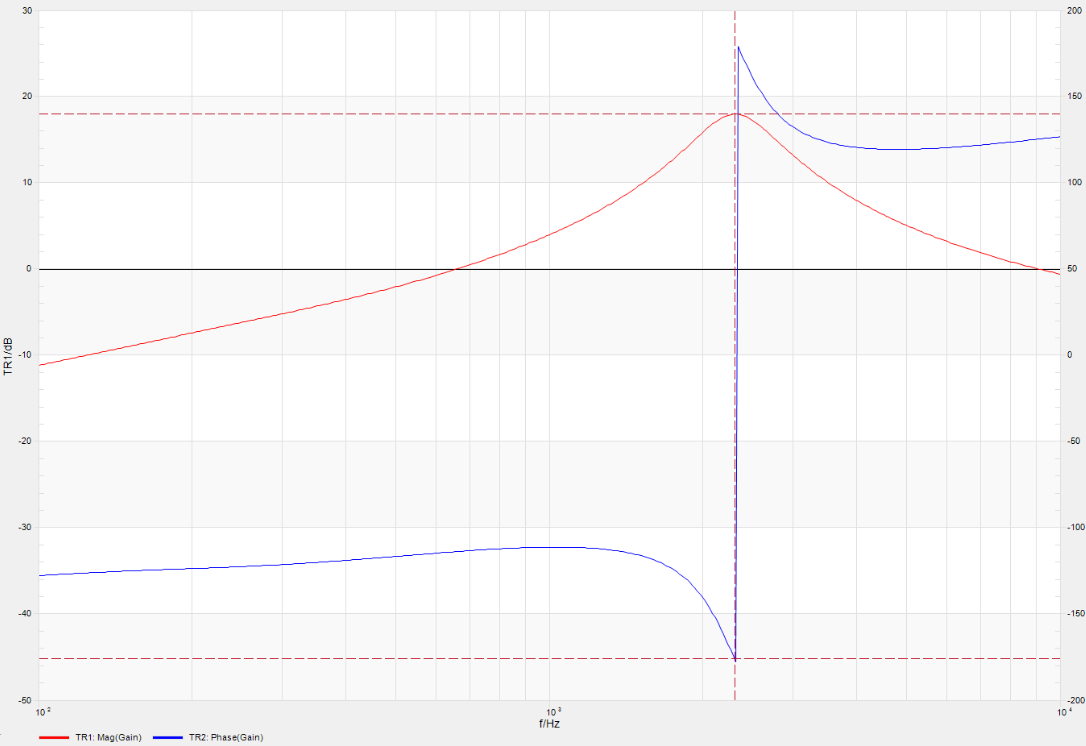
\includegraphics[width=\textwidth]{img/wahwah-2.png}
    \end{subfigure}
    \caption{Measurement of the frequency response of a Wah-Wah-pedal at the lowest and highest frequencies}
    \label{fig:wahwah-filter}
\end{figure}

The resonance frequency of this filter varies between 466\,Hz and 2,3\,kHz.

It is also to be seen, that as the frequency changes, the bandwidth also seem to change. Firstly, it has to be mentioned,
that this is a logarithmic scale. Nevertheless, in an ideal bandpass-filter, the quality factor is constant. This factor indicates
how much energy is dissipated, or how high the loss of a oscillation circuit is. So to keep the Q-factor constant, with
increasing the resonance frequency, the bandwidth also have to increase (\autoref{eq:q-factor}) \cite{taschenbuch_et}.

\begin{align}
    Q = \frac{f_{res}}{f_{3\,dB}}
    \label{eq:q-factor}
\end{align}

By measuring the bandwidths of this filter, it turns out, that the quality factor also changes.

The bandwidth at 466\,Hz is measured to be 54\,Hz, which leads to a Q-factor of:

\begin{align}
    Q = \frac{460\,Hz}{54\,Hz} = 8,518
\end{align}
.

At 2,3\,kHz the bandwidth is 600\,Hz resulting in a quality factor of:

\begin{align}
    Q = \frac{2,3\,kHz}{600\,Hz} = 3,833
\end{align}
.

%// TODO: raus? This behaviour is directly related to how the effect sounds and should therefore be considered in the filter design.

To conclute this, there are two design criteria which can be derived.

\begin{itemize}
    \item mid-frequency varies from 460\,Hz to 2,3\,kHz
    \item it is assumed, that a comparable filter is achieved by using a constant quality-factor of 5
\end{itemize}

\subsubsection{Implementation using \ac{FIR}-filters}

For the first tries, \ac{FIR}-filters were used, because they always guarantee stability \cite{meyer_signalverarbeitung}.
The first prototype of the coefficients combines a set of 32 coefficient sets, which were calculated beforehand
with the following parameters:

\begin{table}[!h]
    \centering
    \caption{Parameters for \ac{FIR}-filterdesign}
    \label{table:fir-filterdesign}
    \begin{tabular}{c | c }
        quality factor & number of coefficients\\
        \hline
        5 & 130
    \end{tabular}
\end{table}

\autoref{fig:wahwah-fir} shows a \ac{FIR}-model of the analog reference at the lowest and (460\,Hz) and the highest
frequency (2242\,Hz).

\begin{figure}[!h]
    \centering
    \begin{subfigure}[c]{0.49\textwidth}
        \centering
        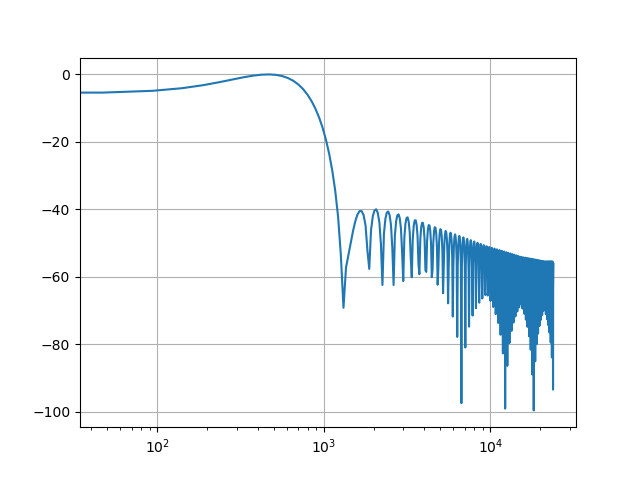
\includegraphics[width=\textwidth]{img/fir_bandpass460.png}
    \end{subfigure}
    \begin{subfigure}[c]{0.49\textwidth}
        \centering
        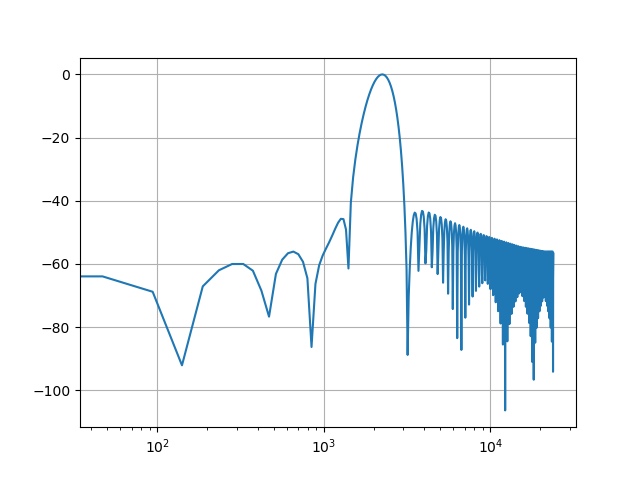
\includegraphics[width=\textwidth]{img/fir_bandpass2242.png}
    \end{subfigure}
    \caption{Simulation of the \ac{FIR}-model frequency response at 460\,Hz and 2242\,Hz}
    \label{fig:wahwah-fir}
\end{figure}

It can be clearly observed, that the shape of the filters are not close to the analog reference.
The filter edges, especially near the baseband, are not steep enough.

\subsubsection{Implementation using biquad-filters}

The second approach to model the filter is by using a biquad-filter \cite{arm_dsp}.
As already mentioned, the filter coefficients are being calculated at runtime.

Therefore following equations are used \cite{cookbook_audio}:

\begin{align}
    \omega_0 = 2 \pi \cdot \frac{f_c}{f_s}\\
    \alpha = \frac{\sin{\omega_0}}{2 \cdot Q}\\
    b_0 = \alpha\\
    b_1 = 0\\
    b_2 = -\alpha\\
    a_0 = 1 + \alpha\\
    a_1 = -2 \cdot \cos(\omega_0)\\
    a_2 = 1 - \alpha
\end{align}

, where $f_c$ is the wanted center frequency, $f_s$ the sampling frequency and $Q$ the quality factor.

Designing a bandpass-filter with a biquad-filter results in the filters shown in \autoref{fig:wahwah-iir}.

\begin{figure}[!h]
    \centering
    \begin{subfigure}[c]{0.49\textwidth}
        \centering
        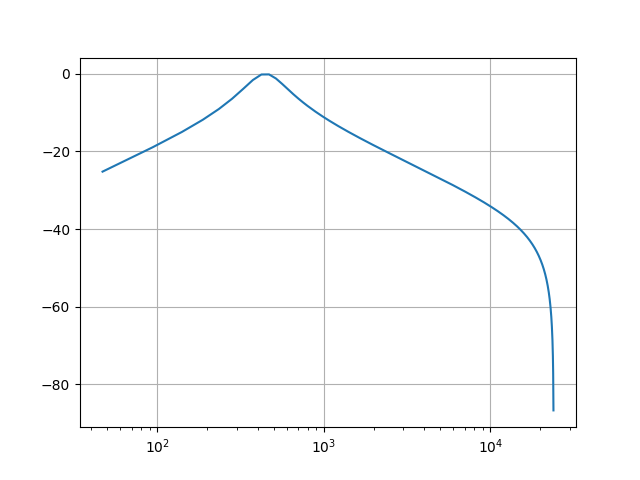
\includegraphics[width=\textwidth]{img/iir_bandpass460.png}
    \end{subfigure}
    \begin{subfigure}[c]{0.49\textwidth}
        \centering
        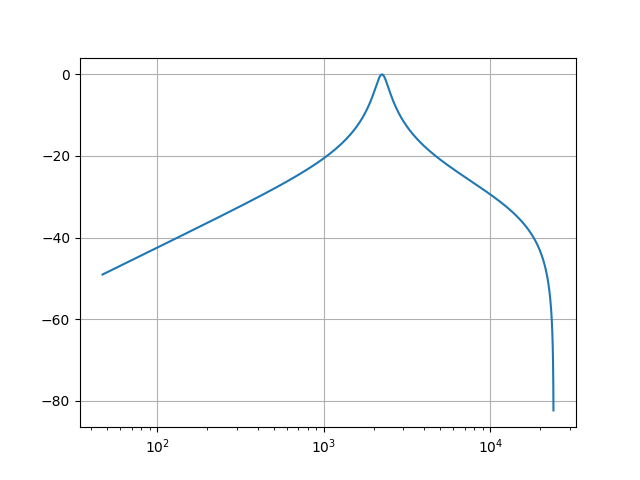
\includegraphics[width=\textwidth]{img/iir_bandpass2242.png}
    \end{subfigure}
    \caption{Simulation of the \ac{IIR}-model frequency response at 460\,Hz and 2242\,Hz}
    \label{fig:wahwah-iir}
\end{figure}

It shows, that the edges of a biquad-filter with five coefficients is much steeper than a \ac{FIR}-filter
with 130 coefficients. In general, the overall shape is closer to the analog reference in comparison to
a non-recursive filter.

\subsection{Evaluation of the filters}

In order to validate, that the implemented filters do in fact emulate a Wah-Wah-effect,
the frequency response is measured as well as running through a hearing test. %// TODO: bessere formulierung

\subsubsection{Evaluation of the \ac{FIR}-filters}

Firstly the \ac{FIR}-filter is evaluated.

To measure the frequency response, an oscilloscope with a signal generator is used. Therefore a sweep
from 50\,Hz to 10\,kHz is applied to the input and a \ac{FFT} of the output is calculated. The result
of the filter at 460\,Hz and 2242\,Hz is shown in \autoref{fig:measure-fir}. On channel 1 (yellow signal)
there is the output and on channel 2 (blue signal) the input signal. The \ac{FFT} result is shown in purple.

\begin{figure}[!h]
    \centering
    \begin{subfigure}[c]{0.49\textwidth}
        \centering
        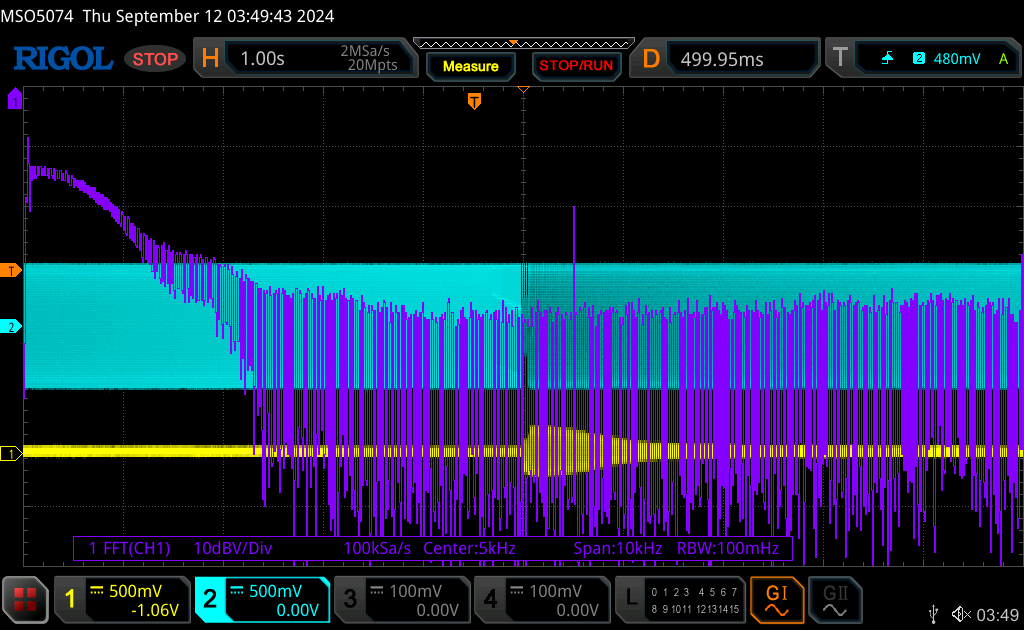
\includegraphics[width=\textwidth]{img/freq_lowest_fir.png}
    \end{subfigure}
    \begin{subfigure}[c]{0.49\textwidth}
        \centering
        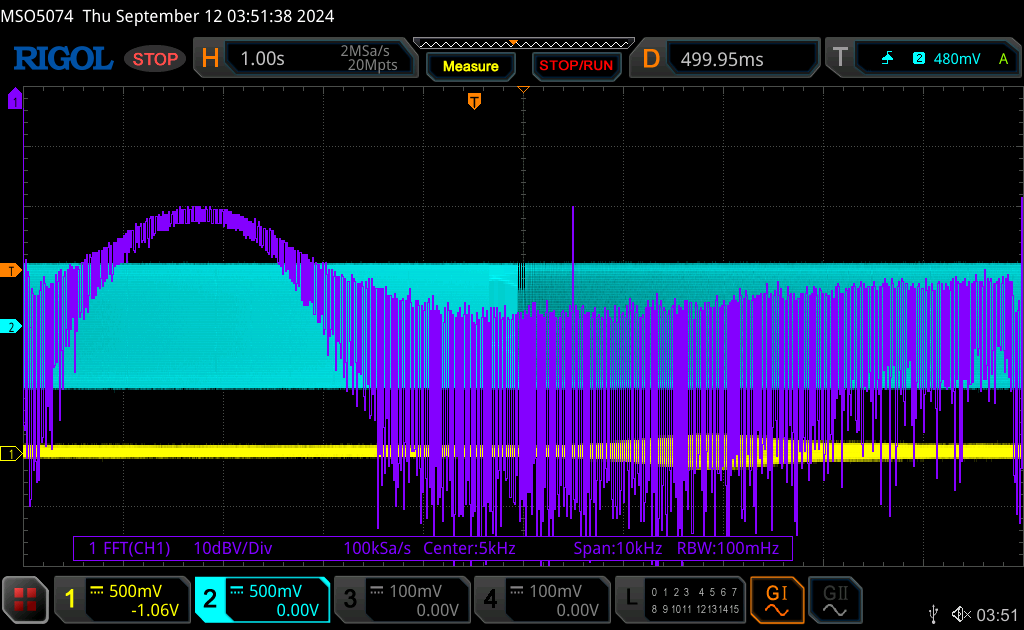
\includegraphics[width=\textwidth]{img/freq_highest_fir.png}
    \end{subfigure}
    \caption{Measurement of the \ac{FIR}-implementation}
    \label{fig:measure-fir}
\end{figure}

The first thing to be recognized is, that the filter at low frequencies is no longer a bandpass, but has
lowpass characteristic. This is expected, if the simulation in \autoref{fig:wahwah-fir} is compared with this result.

Secondly, the filter has flat edges. This is also an expected result.

Lastly, the amplitude in the passband is a fraction of the amplitude of the original signal.
This is not as expected and has to be evaluated in the future. %// evaluate

The first issue that will be recognized, is the cracking noise, when the filter coefficients are being
updated. This can be reduced using fewer filter taps, but the consequence is, a frequency response with
less sharp edges.

The hearing test provides the result, that the sound of this filter emulates a Wah-Wah-effect not sufficiently.



%// TODO: measure, sound of filter

\subsection{Development of the PCB}

In order to get a handy pedal, the whole hardware should be integrated into one single \ac{PCB}.
The dimensions of this should not exceed the standard-sized size of effect pedals. As a reference the
\textit{Boss DS-1} distortion pedal were used to derive a reasonable size for the \ac{PCB}. The dimensions of the
distortion pedal are 73 x 129\,mm, which should not be exceeded. The final \ac{PCB} now has dimensions of
56,39 x 84,33\,mm.

Furthermore, there should be enough inputs, to provide to ability to extend the functionality of this board.
The idea is, to develop a platform, where any effect can be implemented. In order to fulfill this, three analog and
four digital inputs are connected to solderpads for later use. Additionally, an \ac{I2C} connector is also
provided, if for example a little display should be used.

The main components that were chosen are:

\begin{itemize}
    \item STM32H725 microcontroller
    \item CS5343-CZZ Audio \ac{DAC}
    \item CS4344-CZZR Audio \ac{ADC}
\end{itemize}

The reason for the choice of these components is, that the these are also present on the Nucleo- and the
breakout-board. Except for the microcontroller, therefore the smallest package with 68 pins were chosen.

\subsection{Evaluation of the hardware}

There are a few issues on the board, which have been found and fixed so far.

\textbf{Issue 1:}

The first issue is, that the core of the microcontroller is not connected to a source. This is, because
the voltage regulator of this package is not connected to the core. This must be done 
externally. To fix this, a switched-mode power supply was added to the board, which outputs the 1\,V
for the core.

\textbf{Issue 2:}

The output voltage of the extra added power supply is noisy, which led to connection errors with the debugger.
In order to fix this, extra capacitors were added to the supply of the core.

\textbf{Issue 3:}

The input of the op-amp needs an DC-offset voltage as it has only single supply. The offset voltage led
to DC-coupling on the input port. To fix this a decoupling capacitor were added between to the input and the op-amp.

\textbf{Current state:}

It is possible to connect a J-Link debugger to the microcontroller.

%// TODO: picture of pcb
